%csbd_acl

\documentclass[../../main/main.tex]{subfiles}

\begin{document}
\title{Certified Security by Design (CSBD) \& Access\-Control Logic (ACL)}

%%%%%%%%%%%%%%%%%%%%% Chapter CSBD ACL %%%%%%%%%%%%%%%
\chapter[Certified Security by Design (CSBD) \& Access-Control Logic (ACL)]{Certified Security by Design (CSBD)  \\ \& \\ Access-Control Logic (ACL)} \label{chp:csbdacl}


      %%%%%%%%%%%%%%%%%%% Section CSBD %%%%%%%%%%%%%%%%%%
\section{Certified Security by Design (CSBD)} \label{sec:csbd}
In 1970 The Rand Corporation published a report\cite{defensescienceboard} for the Office of The Director of Defense Research And Engineering.  This report titled, Security Controls For Computer Systems, noted that "Providing satisfactory security controls in a computer system is in itself a system design problem."  NIST 800-160 also highlights the importance of incorporating security into the design phase of the system engineering process.  CSBD focuses on the design phase of systems engineering, applying formal methods to verify that a system satisfies the principle of complete mediation.  

More specifically, CSBD is a method for formally verifying and documenting the security properties of a systems.  It focuses on designing systems that satisfy the principle of complete mediation.  It uses an access-control logic (ACL) to reason about access to security sensitive objects of a system.  It uses computer-aided reasoning such as the Higher Order Logic (HOL) Interactive theorem prover to formally verify and document these security properties.  The outcomes of CSBD applied to a system conform to the guidelines set fourth in NIST 800-160 [verify and discuss this.]

In addition to providing formal proofs that demonstrate satisfiability of complete mediation, CDBD is reproducible.  This means that third parties can also verify the formal proofs. This touches on the heart of formal verification of satisfiability: "don't just take my word for it, prove it for yourself."

ACL is described below.  A description of the implementation of ACL in \glsentryshort{hol} is also described below. The implementation of \glsentryshort{acl} is also presented in the appendix in pretty-printed.  The actual HOL code is included with the other files for this master thesis.  It is included under /MasterThesis/HOL/ACL.

      %%%%%%%%%%%%%%%%%%% Section ACL %%%%%%%%%%%%%%%%%%%
\section{Access-Control Logic (ACL)} \label{sec:acl}

\subsection{ACL: A Command and Control (C2) Calculus} \label{ssec:aclc2}
\glsentryshort{acl} is a logic for reasoning about access to object.  In the jargon of the day it is a command and control (C2) calculus\footnote{command and control being self-evident and calculus being a method for reasoning}.  All the axioms and definitions described above are implemented in the \glsentryshort{acl}.  The actual code is included with the files for this thesis.  A pretty-printed print-out of the \glsentryshort{acl} is included in appendix \ref{ppacl}.

\subsection{Principals}\label{ssec:principals}
Principals should be thought of as actors in the access-control logic.  Principals can make statements or requests.  They can be assigned privileges or authority over objects or actions.  The text defines allowable principals using the identifier \textbf{Princ}:


\begin{center}
\textbf{Princ ::= PName / Princ \& Princ / Princ \textbar  Princ}\label{Princ}
\end{center}

This is a recursive definition. \textbf{\textit{PName}} refers to the name of a principal (i.e., Jane, PlatoonLeader, sensor1).  \textbf{\textit{Princ} \& \textit{Princ}} is read "Princ with Princ" or "Princ and Princ" (i.e., Principal1 with Principal2). \textbf{\textit{Princ \textbar  Princ}} is read as "Princ quoting Princ" (i.e., Principal1 quoting Principal2).


\subsection{Propositional Variables, Requests, Authority, and Jurisdiction}\label{ssec:statementsacl}
To reason about access-control and trust, the \glsentryshort{acl} uses propositional variables, requests, authority, and jurisdiction to make statements.

Propositions in logic are assertions that are either true or false.  For example, "I am reading this master thesis" is a proposition because either you are or you are not reading this.  Propositional variables are just place holders for propositions.  For example, "I am reading something", where the propositional variable "something" is what you are reading.

Principals can make requests.  In the \glsentryshort{acl}, principals make requests using the \textit{says} operator.  Requests have the form \textit{P says $\varphi$},  where \textit{P} represents some principal and \textit{$\varphi$} represents some assertion.  For example, \textit{PlatoonLeader says platoonHalt}.  In this example, the Platoon Leader is issuing a command (or request) for the platoon to halt.  

Principals can have authority over assertions.  In the \glsentryshort{acl}, authority is conveyed using the \textit{controls} operator.  Statements of authority have the form \textit{P controls $\varphi$},  where \textit{P} represents some principal and \textit{$\varphi$} represents some assertion.  For example, \textit{PlatoonLeader controls platoonHalt}.  This example states that the Platoon Leader has the authority to issue the command (or request) for the platoon to halt. 

Principals can also have jurisdiction over assertions.  Both authority and jurisdiction use the \textit{controls} operator.  Statements of jurisdiction have the same form as statements of authority.  Statements of authority are typically defined in an organization's policy.  Statements of jurisdiction are statements that are readily believed given the context.  For example, \textit{PresidentOfUS controls (PlatoonLeader controls platoonHalt)}.  In this example, the President of the United States, per the U.S. Constitution, has jurisdiction over the authority invested in the Platoon Leader.  In particular, the President of the United States has the jurisdiction to give the Platoon Leader the authority to command her platoon to halt.

In addition, principals can speak for other principals.  Principals do this using the \textit{speaks for} operator.  The ACL represents the \textit{speaks for} operator with the symbol $\Rightarrow$.  These types of statements have the form \textit{P $\Rightarrow$ Q}, where both \textit{P} and \textit{Q} are principals.  For example, \textit{PlatoonLeader $\Rightarrow$ PresidentOfUS}.  This example states that the Platoon Leader speaks for the President of the United States.  

\subsection{Well-formed Formulas}\label{ssec:wff}
\Glspl{wff} define the syntax (or grammatical structure) of the propositional logic.  They are valid statements in the \glsentryshort{acl}.  All \glsentryshort{ACL} statements must be a \glsentryshort{wff}.  The text book defines the set of \glsentryshortpl{wff} using the identifier \textbf{Form}:

\begin{center}
\textbf{Form} ::= \textbf{PropVar} / $\neg$ \textbf{Form} / (\textbf{Form} $\vee$ \textbf{Form}) / \\ 
	                  (\textbf{Form} $\wedge$ \textbf{Form}) / (\textbf{Form} $\supset$ \textbf{Form}) / (\textbf{Form} $\equiv$ \textbf{Form}) / \\
	                  (\textbf{Princ} $\Rightarrow$ \textbf{Princ}) / (\textbf{Princ} says \textbf{Form}) / (\textbf{Princ} controls \textbf{Form}) /\\
	                  (\textbf{Princ} reps \textbf{Princ} on \textbf{Form}\footnote{The last line is from \cite{certmanual}.})
\end{center}

This is a recursive definition.  \textbf{\textit{PropVar}} is a propositional variable.  The symbols $\neg$, $\vee$, $\wedge$, $\subset$, and $\equiv$ are the standard set and logical symbols.  They represent "not", "or", "and", "implication", and "equivalence", respectively.  

\subsection{Kripke Structures \& Semantics}\label{ssec:kripke}
Kripke structures are named after Saul Kripke.  Kripke is an influential figure in logic and philosophy.  He is recognized, in particular, for inventing the Kripke semantics for modal logic \cite{saulk}.    

Whereas \glsentryshortpl{wff} define the syntax of the propositional logic, Kripke semantics describe the semantics.  Semantics refers to the meaning of statements.  In propositional logic, \glsentryshortpl{wff} can be either true or false.  

\subsubsection{Kripke Structures}
Before defining the Kripke semantics, the concept of a Kripke structure is necessary.  A Kripke structure primarily deals with three things: worlds, propositions, and principals.  The worlds can be thought of as possible states or configurations of some system.  Propositions are just statements that are either true or false.  And, principals are just actors.  A Kripke structure $\mathcal{M}$ = $\langle \textit{W}, \textit{I}, \textit{J} \rangle $  is defined as a three-tuple consisting of the following: a set of worlds \textit{W}; a function \textit{I} called the assignment function that maps propositions to worlds, and ; a function \textit{J} that maps principals to relations on worlds, where the relation is called the accessibility relation.  Formally, these are defined as follows (definition 2.1 in the text): 

\begin{itemize}
\item \textit{W is a nonempty set, whose elements are called worlds.}
\item \textit{$I: \mathbf{PropVar} \rightarrow \mathcal{P}(W)$ is an interpretation function that maps each propositional variable to a set of worlds.}
\item \textit{$J: \mathbf{PName} \rightarrow \mathcal{P}((W \times W)$ is a function that maps each principal name to a relation on worlds.}
\end{itemize}

One way to think of Kripke structures is as a logic on multiple worlds or possible states.  For example, consider two planets Earth and Tatooine\footnote{Tatooine is the fictional home planet of Luke Skywalker.  Tatooine has two suns.  \cite{Tantooine}}.  Let $\varphi$ be the proposition "this is planet Tatooine" and $\theta$ be the proposition "this is a planet."  Then $I(\varphi) = \{Tatooine\}$ and $I(\theta) = \{Earth, Tatooine\} = W$, where \textit{W} is the set of all worlds (\{Earth, Tatooine\}).  Furthermore, let "Luke" and "Lea" and "Uncle Owen" be principals.  Now consider the following:  Luke can get from Earth to Earth and from Tatooine to Earth (and vis-a-vis).  He can also get from Tatooine to Tatooine.  Lead can get from Earth to Earth and from Tatooine from Earth.  But, she can not get from Tatooine to Tatooine.  Uncle Owen can only get from Tatooine to Tatooine.  He can not get to Earth.  Then, $J(Luke) = \{(Earth, Earth),(Earth, Tatooine),(Tatooine, Earth), (Tatooine, Tatooine)\}$.  $J(Lea) = \{(Earth, Earth),(Earth, Tatooine),(Tatooine, Earth)\}$. And, $J(Uncle Owen) = \{(Tatooine, Tatooine)\}$. With \textit{W}, \textit{J}, and \textit{I} defined, this forms a Kripke structure.



Kripke structures are necessary to define the ACL properly.  In particular, they are necessary to define the concepts of "satisfies" and "soundness" which follow.  However, an in-depth understanding of Kripke structures is not necessary to understand the work in this master thesis.  

\subsubsection{Kripke Semantics}
The Kripke semantics define the meanings of \glsentryshortpl{wwf} for Kripke structures.  The semantics can be thought of as an evaluation function for a particular Kripke $\mathcal{M}$ = $\langle \textit{W}, \textit{I}, \textit{J} \rangle $.  Figure \ref{kripkesemantics} shows the Kripke semantics.  The subscript $\mathcal{M}$ signifies that the evaluation function is defined for a particular Kripke structure.  This means there is a separate evaluation function for each Kripke structure.


\begin{figure}[h]
\centering
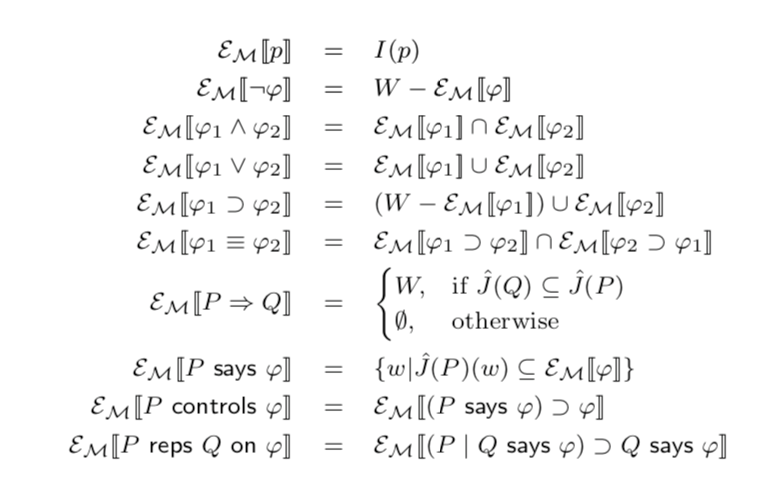
\includegraphics{../figures/kripkesemantics}
\caption{\label{kripkesemantics} Kripke semantics. Image taken from \textit{Access Control, Security, and Trust: A Logical Approach}\cite{ChinOlder}}
\end{figure}

For example, for the Kripke structure described above, $\varepsilon_{\mathcal{M}}\textlbrackdbl \varphi \textrbrackdbl  = \{Tantooine\}$ and $\varepsilon_{\mathcal{M}}\textlbrackdbl \theta \textrbrackdbl  = \{Earth, Tantooine\} = W$ (the set of all worlds).  As an another example, $\varepsilon_{\mathcal{M}}\textlbrackdbl \text{Luke says $\varphi$} \textrbrackdbl = \{Earth, Tatooine\}$\footnote{Think about it.  }

\subsubsection{Satisfies}\label{sssec:satisfies}
The "satisfies" condition applies to a particular Kripke structure $\mathcal{M}$ = $\langle \textit{W}, \textit{I}, \textit{J} \rangle $.  It is said the $\mathcal{M}$ satisfies some proposition $\varphi$ if the evaluation function $\varepsilon_{\mathcal{M}}\textlbrackdbl \varphi \textrbrackdbl = W$ (the set of all worlds) for  $\mathcal{M}$.  In other words, $\varphi$ is true in all worlds of $\mathcal{M}$.  Symbolically, this is denoted as $\mathcal{M} \models \varphi$.  The statement $\mathcal{M}$ does not satisfy $varphi$ is denoted as $\mathcal{M} \not\models \varphi$.

In the example above, the Kripke structure $\mathcal{M} \models \theta$, where $\theta =$ the proposition "this is a planet."

\subsubsection{Soundness}\label{sssec:soundness}
Whereas "satisfies" describes a property of a Kripke structure $\mathcal{M}$, "soundness" describes a property of all Kripke structures. 

Soundness refers to the logical consistency of inference rules.  Inference rules consist of a set of hypothesis \{$H_1, H_2, \dots , H_n$\} and a conclusion. 
\begin{equation*}
\frac{H_1, H_2, \dots , H_n}{C}
\end{equation*}

An inferences rule is said to be sound if for every Kripke structure $\mathcal{M}$ that satisfies all the hypothesis, the conclusion is true. In other words,  the inference rule is sound if and only if $\forall H_i, \mathcal{M} \models H_i \longrightarrow \mathcal{M} \models C$.

Soundness is verified by formal proofs that employ axioms, tautologies, and sound inference rules that are already proved.  

\subsection{Inference Rules}\label{ssec:inferencerules}
The inference rules for the \gls{acl} are shown in figure \ref{inferencerules}.  All the inference rules are sound.  Details of proofs of soundness can be found in \textit{Access Control, Security, and Trust: A Logical Approach}\cite{ChinOlder}.

\begin{figure}[h]
\centering
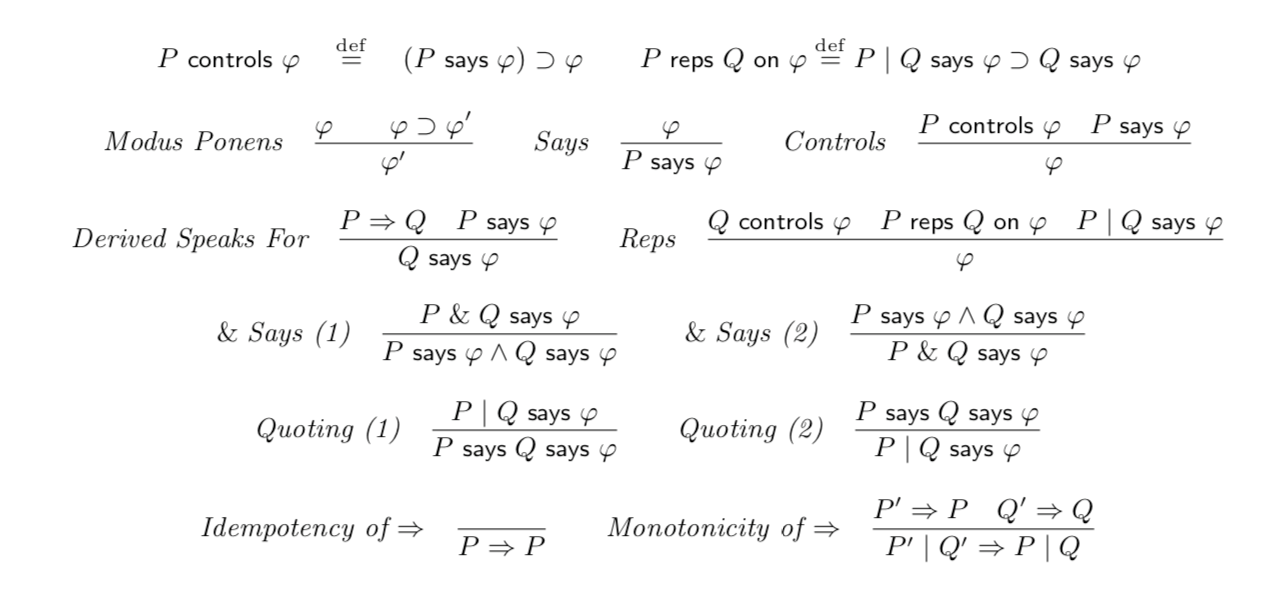
\includegraphics[width=\textwidth]{../figures/inferencerules}
\caption{\label{inferencerules}The \gls{acl} inference rules. Image taken from \textit{Access Control, Security, and Trust: A Logical Approach}\cite{ChinOlder}}
\end{figure}

\subsection{Complete mediation}\label{ssec:aclcompletemediation}
Fundamental to this work is the concept of complete mediation (discussed in section \ref{ssec:pcompletemediation}).  In the \glsunset{acl}\gls{acl}, this means that each principal must be authenticated and authorized on each request.   ACL does this primarily by the \textit{Controls} inference rule in figure \ref{inferencerules} and shown again here in figure \ref{ControlsInferenceRule}. 

\begin{figure}[h]
\centering
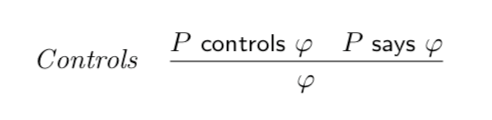
\includegraphics{../figures/ControlsInferenceRule}
\caption{\label{ControlsInferenceRule}The \textit{Controls} inference rule. Image taken from \textit{Access Control, Security, and Trust: A Logical Approach}\cite{ChinOlder}}
\end{figure}

ACL refers to the left statement as an authorization\footnote{or a \textit{control} in the C2 calculus}.  The principal P controls (is authorized on) some action $\varphi$. ACL refers to the right statement in this inference rule as a request \footnote{or a \textit{command} in the C2 calculus}.  The principal P requests some action $\varphi$. The conjunction of the authorization and the request of P on $\varphi$ results in the action $\varphi$.  That is, if \textit{P controls $\varphi$} and\textit{ P says $\varphi$} then $\varphi$  is true.  

The \textit{Controls} rule is sufficient for basic authorization involving one principal and some action.  It is the only rule applied in this master thesis.  But, there are more complicated rules that allow for additional authentication and authorization schemes.  

\begin{figure}[h]
\centering
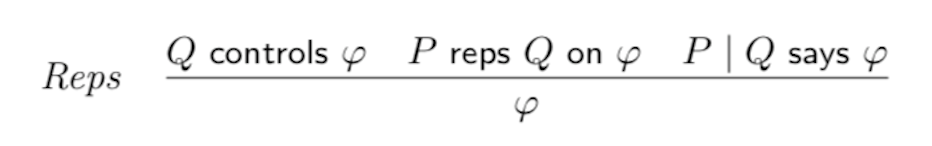
\includegraphics[width =0.7 \textwidth]{../figures/repsrule}
\caption{\label{repsrule}The \textit{Reps} inference rule. Image taken from \textit{Access Control, Security, and Trust: A Logical Approach}\cite{ChinOlder}}
\end{figure}

The \textit{Reps} (shown in figure \ref{repsrule}) rule also demonstrates complete mediation.  It follows a similar logic.  But, this rule has two principals, in this case P and Q.  The idea is that Q controls (is authorized on) some action $\varphi$. And also, P represents Q on that action.  In the \glsentryshort{acl}, this means that \textit{P Reps Q on $\varphi$}.  Thus, \textit{P says $\varphi$} is irrelevant because P does not have authority on $\varphi$.  But, \textit{P \textbar Q says $\varphi$} (short for, \textit{P says Q says $\varphi$}) is relevant because P represents Q and Q has authority.  Spelled out, the rule follows as such: if \textit{Q controls $\varphi$ and P reps Q on $\varphi$ and P \textbar Q on $\varphi$} then $\varphi$ is true.

The \textit{Reps} rule represents a principal acting in a role.  For example, soldier G.I. Jane may be acting as the Platoon Leader.  In this situation, it is the Platoon Leader (Q) who is granted authority over the action $\varphi$.  But, it is G.I.Jane (P) acting in the role of Platoon Leader who (Q) is actually issuing the command $\varphi$.  

\begin{figure}[h]
\centering
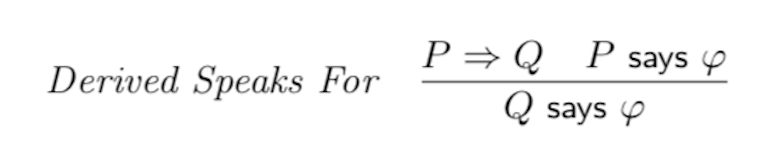
\includegraphics[width =0.6 \textwidth]{../figures/derivedspeaksfor}
\caption{\label{derivedspeaksfor}The \textit{Derived Speaks For} inference rule. Image taken from \textit{Access Control, Security, and Trust: A Logical Approach}\cite{ChinOlder}}
\end{figure}

The \textit{Derived Speaks For} rule also allows for variation in authentication and authorization. This rule is shown in figure \ref{derivedspeaksfor}. This also uses two principals and deals mainly with the concept of jurisdiction and authentication.  In this case, the principal P is "speaking for" the principal Q.  Again, the symbol $\Rightarrow$ means "speaks for."  Thus, if \textit{P $\Rightarrow$ Q and P says $\varphi$} then we believe that \textit{Q says $\varphi$}.

The most common use of the \textit{Derived Speaks For}  rule is in jurisdictional case.  For example, the United States Army has jurisdiction over who serves in the role of Platoon Leader.  The U.S. Army may, in turn, issue i.d. cards with a soldier's photo (or in the future chips) that say, for example, soldier G.I.Jane is who the she says she is.  If we believe the i.d. card is genuine and it belongs to G.I.Jane, then the  i.d. card speaks for G.I.Jane.  So, if the i.d. card says issue G.I.Jane her equipment, then it follows that G.I. Jane says to issue her the equipment.  It is somewhat more complicated, because the U.S. Army has jurisdiction over who gets what equipment.  The i.d. card is not saying that G.I.Jane has control over her equipment.  It only says that she is asking for the equipment.  

The \textit{Derived Speaks For} rule is critical to authentication, whereas the \textit{Controls} and \textit{Reps} rules are critical for authentication.


      %%%%%%%%%%%%%%%%%%% Section ACL in HOL %%%%%%%%%%%%%%%
\section{ACL in HOL} \label{sec:aclinhol}
The material in this section is adapted from \textit{Access Control, Security, and Trust: A Logical Approach}\cite{ChinOlder} and \textit{Certified Security by Design Using Higher Order Logic}\cite{certmanual}. In this section, the former is referred to as "the text" and the later is referred to as "the manual."


This section describes how the access-control logic (\glsentryshort{acl}) is implemented in the Higher Order Logic (\glsentryshort{hol}) Interactive Theorem Prover.
The goal is to describe the implementation in sufficient detail that the reader can understand the descriptions of the patrol base operations that follow in this thesis. 


\subsection{Principals}
Figure \ref{princHOL} shows the \glsentryshort{hol} representations for principals (\textbf{\textit{Princ}}).

\begin{figure}[h]
\centering
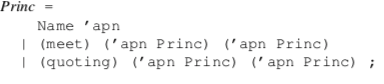
\includegraphics[width=0.6\textwidth]{../figures/princHOL}
\caption{\label{princHOL}The HOL implementations of principle (\textbf{\textit{Princ}}).  Image from  \textit{Certified Security by Design Using Higher Order Logic}\cite{certmanual}}.  
\end{figure}

The concept of types are important in \glsentryshort{hol}.  They are discussed in the background chapter in section \ref{adt}.  \textbf{\textit{Princ}} is an algebraic data type.  

The first thing to notice about  \textbf{\textit{Princ}} is that there are three definitions just as there are in the definition of  \textbf{\textit{Princ}} in section \ref{Princ}.   The first line within the definition above corresponds to \textbf{\textit{PropVar}}, the second corresponds to \textbf{Princ \& Princ}, and the third corresponds to \textbf{Princ \textbar  Princ}.  In \glsentryshort{hol} the infix \& operator is represented with the prefix \texttt{meet} operator.  The infix \textbar operator is represented with the prefix \texttt{quoting} operator.

The primary difference between datatype definitions in \glsentryshort{hol} and ML (the metalanguage in which \glsentryshort{hol} is implemented) is that \glsentryshort{hol} does not use the keyword "of" before the type definition.  Thus, the first line of this definition is \texttt{Name 'apn} and not \texttt{Name of 'apn}.  As in ML, forward tick marks (apostrophes) always precede a type variable. 


In the definition for  \textbf{\textit{Princ}}, \texttt{Name} is called the type constructor.  The result of the constructor and a concrete type or type variable results in something of type \textbf{\textit{Princ}}.  Examples of principals defined in \glsentryshort{hol} take the following form.
\[Name PlatoonLeader, or \]
\[(Name PlatoonLeader) \textasciigrave meet ` (Name PlatoonSergeant), or \]
\[(Name PlatoonLeader) `quoting` (Name PlatoonSergeant). \]

Prefix operators may be used as infix operators if they are surrounded by the back tick (typically located near the esc-key). This master thesis focuses on principals defined using the \texttt{Name PlatoonLeader} construction. 

\subsection{Kripke structures}



Kripke structures are part of the implementation of the \glsentryshort{acl} in \glsentryshort{hol} because they are necessary to prove the "satisfies" and "soundness" properties of the \glsentryshort{acl}.  Nevertheless, the model of patrol base operations does not require any definition of a Kripke structures.   For the most part, Kripke structures in \glsentryshort{hol} are coded as (M, Oi, Os), where M represents the Kripke structure and Oi and Os represent the integrity and security levels (not used in this master thesis).  A more properly typed coding of the Kripke structure has the form \[ \texttt{M:('prop, 'world,'pName, 'Int, 'Sec)Kripke, (Oi: 'Int po), (Os:'Sec po)} \].

\textbf{\textit{Princ}} is the type definition.  

The definition of \textbf{Form} (described above) in the \glsentryshort{acl} is shown in figure ref{FormACL}.

\begin{figure}[h]
\centering
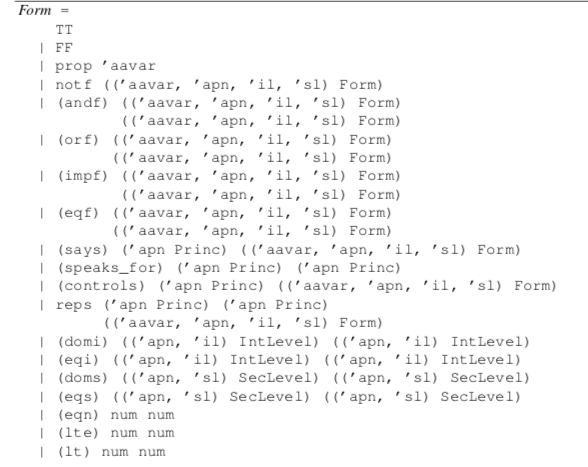
\includegraphics[width=\textwidth]{../figures/FormACL}
\caption{\label{FormACL}The definition for \textbf{Form} in HOL.   \textit{Certified Security by Design Using Higher Order Logic}\cite{certmanual}}
\end{figure}

\textbf{Form} is a datatype definition.  Recall from the Background section that \glsentryshort{hol} is a strongly-typed language.   

\texttt{TT}  and \texttt{FF} are the \glsentryshort{acl} representations of true and false, respectively.  \texttt{prop 'aavar} is the equivalent of \textit{\textbf{ProVar}} in the definition for \textbf{Form}.  The first part \texttt{prop} is called the type variable.  \texttt{prop 'aavar} is a type variable.  \glsentryshort{hol} is a strongly-typed language.  The type variable tells \glsentryshort{hol} what types are associated with a datatype of


\glsentryshort{hol} can often figure out what the type of a specific definition is.  But, one quickly learns when working with \glsentryshort{hol} is that its best to be explicit when it comes to types.  

The equivalence of the \gls{acl} formulas implemented in HOL are shown in figure \ref{aclformulasHOL}.

\begin{figure}[h]
\centering
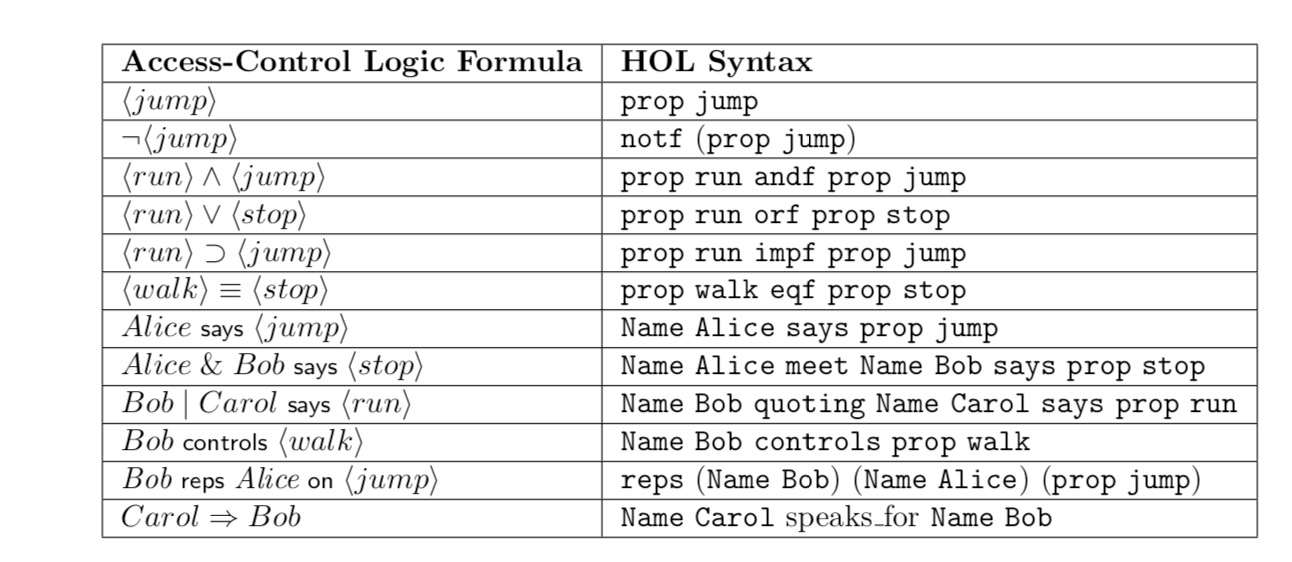
\includegraphics[width=\textwidth]{../figures/aclformulasHOL}
\caption{\label{aclformulasHOL}The \gls{acl} formulas in HOL.  Image taken from \textit{Access Control, Security, and Trust: A Logical Approach}\cite{ChinOlder}}
\end{figure}

Using this syntax, an ACL request takes the form \textit{P says \textphi} \centerline{ \textit{Name P says prop \textphi}}


\subsection{Complete Mediation}
\subsection{satList}


\end{document}
